% iaus2esa.tex -- sample pages for Proceedings IAU Symposium document class
% v1.04,  Copyright (2004) International Astronomical Union

\NeedsTeXFormat{LaTeX2e}

\documentclass{iau}
% Include figures (EPS only), using e.g.:
\usepackage{graphicx} 


%% -- Title ------------------------------------
\title[Multiwavelngth Astronomy ~~PSR J0737$-$3039] %% short title %%
{Using the Universe as a Physics Laboratory: A Multiwavelength Review of PSR J0737$-$3039} %% full title %%

%% -- Authors ----------------------------------
\author[Umang Mishra]  %% short author list %%
{Umang Mishra $^1$}
% \thanks{Present address: ...},
%% \and Author Two$^2$}

\affiliation{New York University Abu Dhabi\\ email: {\tt um339@nyu.edu}} 
%%\\[\affilskip]
%%$^2$A, \\ B \\email: {\tt c@d.com}}

%% -- Header (pre-filled, do not edit) -----------------
%\pubyear{2012}
%\volume{1}  %% insert here IAU Symposium No.
% \pagerange{1--9}
% \date{?? and in revised form ??}
% \setcounter{page}{1}
%\jname{\mbox{Multi-Wavelength Astronomy: Final Reports of Sources Studied in Depth}}
%\editors{M. S. E. Roberts , ed.} 
\begin{document}

\maketitle

%% -- Abstract ----------------------------------
\begin{abstract}

This paper is a multi-wavelength review of the double pulsar binary PSR J0737$-$3039. 
(more will be added once the entire paper is finished).

%% add here a maximum of 10 keywords, to be taken form the file <Keywords.txt>
\keywords{PSR J0737$-$3039,Double Pulsar Binary, General Relativity}
\end{abstract}

% add below any authors, subjects and objects for indexing 
%   add more lines if necessary
%   but leave all lines commented out
%\index[author]{LastName1, Initials|textbf}
%\index[author]{LastName2, Initials|textbf}
%\index[subject]{Keyword1}
%\index[subject]{Keyword2}
%\index[object]{Object1}
%\index[object]{Object2}


\firstsection % if your document starts with a section,
              % remove some space above using this command.
\section{Introduction}
The double pulsar binary system J0737$-$3039 was discovered in 2004 using the Parkes 64-m radio telescope in New South Wales, Australia by \cite{b03}. Right from its discovery, the pulsar binary was anticipated to be crucial towards better understanding of  Post Newtonian formalism and gravitational waves. J0737$-$3039A is a millisecond pulsar with 22.7ms period, and its counterpart is a young unrecycled pulsar with a period of 2.77 s as summarized by \cite{lyn06} . While initially the system was only observed in the radio wavelengths for testing general relativity, observations were also performed using XMM Newton in soft X-ray. Some observations in gamma ray have also been performed. (More info on X-Ray and gamma later)

\section{Radio Observations}

\subsection{The Discovery and the Parameters}
Although the first observation was made by the Parkes 64-m at 1390Hz, better precision was obtained after interferometric observations were made using the Australia Telescope Compact Array(ATCA). The pulsar A of the system was found to be in a 2.4 hour eccentric orbit with eccentricity of 0.088 by \cite{b03}. The ATCA measurements helped further measurement of parameters, giving a period of 22.699 ms for pulsar A. The period of pulsar B was found to be 2.8s by \cite{lyn04}.
 
The periastron advance($\dot\omega$) value was measured to be 16.88yr$^{-1}$ by the ATCA observations. This was the highest value of $\dot\omega$ and was used to predict the masses of the pulsars in the system.\cite{lyn04} also measured other post Keplerian parameters, and found that the predictions of masses were accurate. The system was thus established as a highly relativistic double pulsar binary system ideal for testing relativistic gravity and DNS merger rates.

\subsection{The Double Neutron System(DNS) as a Testing Ground for General Relativity}

\begin{figure}[h!]
	\begin{center}
		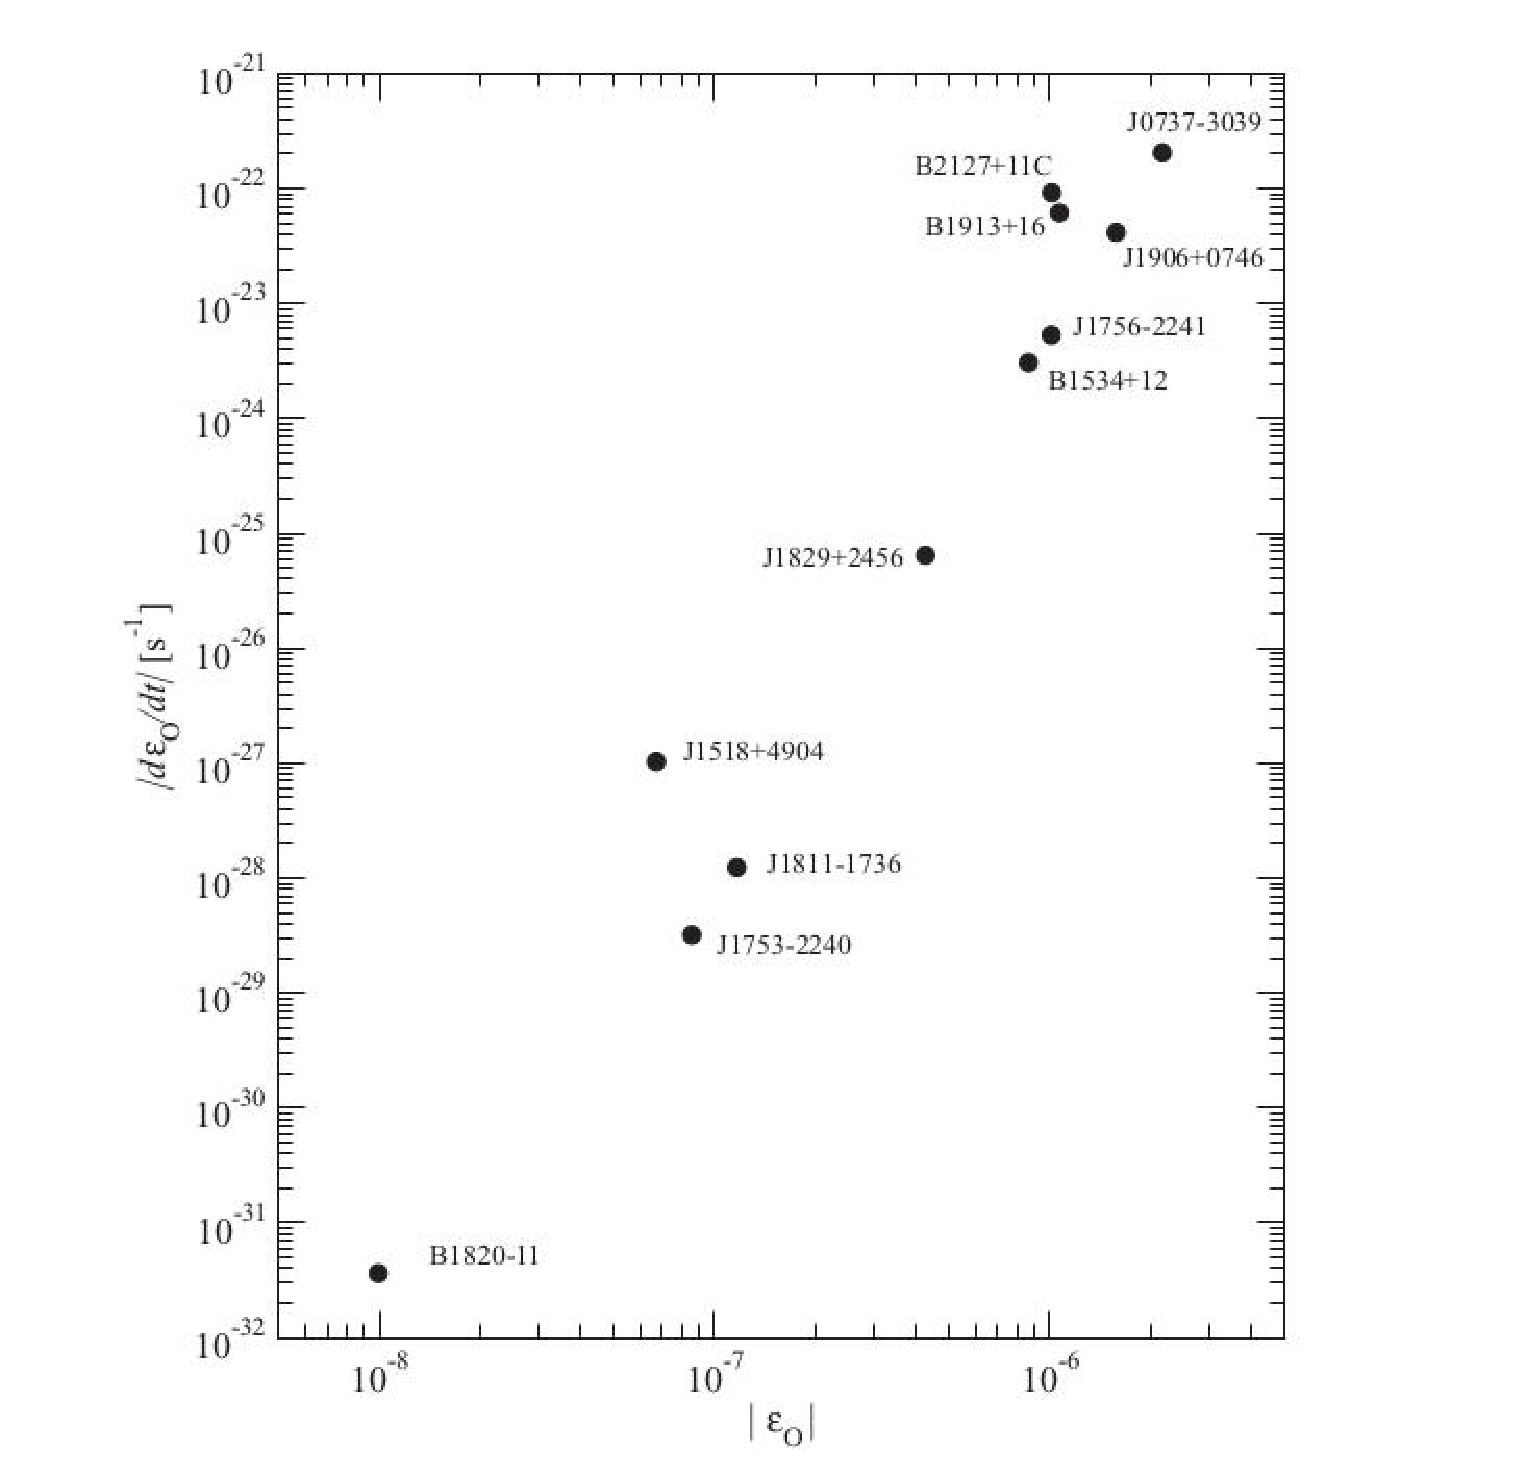
\includegraphics[width=3.4in]{fig1.eps} 
		\caption{Orbital energy-energy loss diagrams for known and likely double neutron binaries. $\epsilon_o$ is a direct measure for the strength of post-Newtonian effects in orbital dynamics. It can thus clearly be seen that J0737-3039 (top right) is the most suitable candidate for studying relativistic gravity. Image taken from \cite{kwex09} }
		\label{fig1}
	\end{center}
\end{figure}

Usually, five Keplerian Parameters are sufficient to describe binary systems. These are: P$_{orb}$, e, $\omega$, a$sin i$, and T$_o$. In case of strong gravitational interactions, such as in the case of a double neutron system, six additional parameters called the post-Keplerian parameters are required to fully describe the system due to relativistic effects that come into play. These are : $\dot\omega$, $\gamma$, $r$, $s$,dP$_b$/dt, and $\Omega_{SO}$. Since gravity is the only way stars in DNS interact, it makes them ideal candidates for studying relativistic gravity theories using these post-Keplerian parameters. The description of these parameters can be found in table 1. 

\begin{table}[]
	\centering
	\caption{A description of the six post-Keplerian parameters}
	\begin{tabular}{p{1cm}|p{3cm}|p{8cm}}
		\hline
		$\dot\omega$  & Periastron advance                     & Describes the rotation of the line connecting two pulsars at their closest approach to each other                        \\ \hline
		$\gamma$      & Gravitation Redshift and Time Dilation & Accounts for the apparent slowing of time due to general and special relativistic effects                                \\ \hline
		$r$ and $s$   & Shapiro Delay                          & These parameters define the Shapiro delay, which is delay in receiving signal due to space-time curvature                \\ \hline
		dP$_b$/dt     & Orbital Decay                          & The rate of decrease of the orbital period due to emission of gravitational waves                                        \\ \hline
		$\Omega_{SO}$ & Relativistic Spin Precession           & Rate of the apparent precession of the pulsar about the orbital angular momentum that arises due to space-time curvature \\ \hline
	\end{tabular}
\end{table}

As shown in figure 1, PSR J0737-3039 is the most suitable system for studying relativistic gravity.  Each of the post-Keplerian(PK) parameters is related to the masses of the pulsars in the system in a unique way.With a system as J0737-3039, a ratio of stellar masses can be obtained from observations and plotted as a straight line according to the equation: \[\frac{a_B sini}{a_A sini}=\frac{m_A}{m_b}\]
An intersection between this line and the curves plotted for each PK on a mass-mass plot could be used as a verification test for general relativity. 

In the case of PSR J0737-3039, all five PK parameters can be measured for pulsar A. Since the equations for $\dot\omega$, $s$, and dP$_b$/dt for general relativity are symmetric in masses, they will be the same for both pulsar A and pulsar B. Studies of eclipses of A allow for measurement of $\Omega_{SO}$ for B. The mass-mass plot for these parameters, can be seen in figure 2. While all the experimental values agree within the error boundaries with the theoretical predictions, the best match is with Shapiro delay(with uncertainty of 0.05\%). Exact values are listed in table 2.

\begin{table}[]
	\centering
	\caption{A comparison of measured and predicted values of the six post-Keplerian parameters. Values taken from \cite{kwex09}}
	\begin{tabular}{p{3cm} p{3cm} p{3cm} p{3cm}}
		\hline
		Parameter & Observed value & GR expectation & Ratio  \\ 
		\hline
		$\dot\omega$ (deg yr$^{-1}$)  &    16.899 47(68) & - & -  \\ \hline
		$\gamma_A (ms) $     &  0.3856(26) & 0.38418(22) &  1.0036(68)   \\ \hline
		$r_A$ ($\mu$s)  & 6.21(33) &  6.153(26) & 1.009(55) \\ 
		\hline
		$s$  &0.999 74(−39, +16)&  0.999 87(−48, +13)&0.999 87(50) \\ 
		\hline
		dP$_b$/dt     & 1.252(17) & 1.24787(13) & 1.003(14)  \\ 
		\hline
		$\Omega_{SO}$ (deg yr$^{-1}$) & 4.77(+0.66, −0.65)  &  5.0734(7) & 0.94(13)  \\ \hline
	\end{tabular}
\end{table}


% CUP work flow only accepts EPS -- not PDF, JPG, etc.
\begin{figure}[h!]
	\begin{center}
		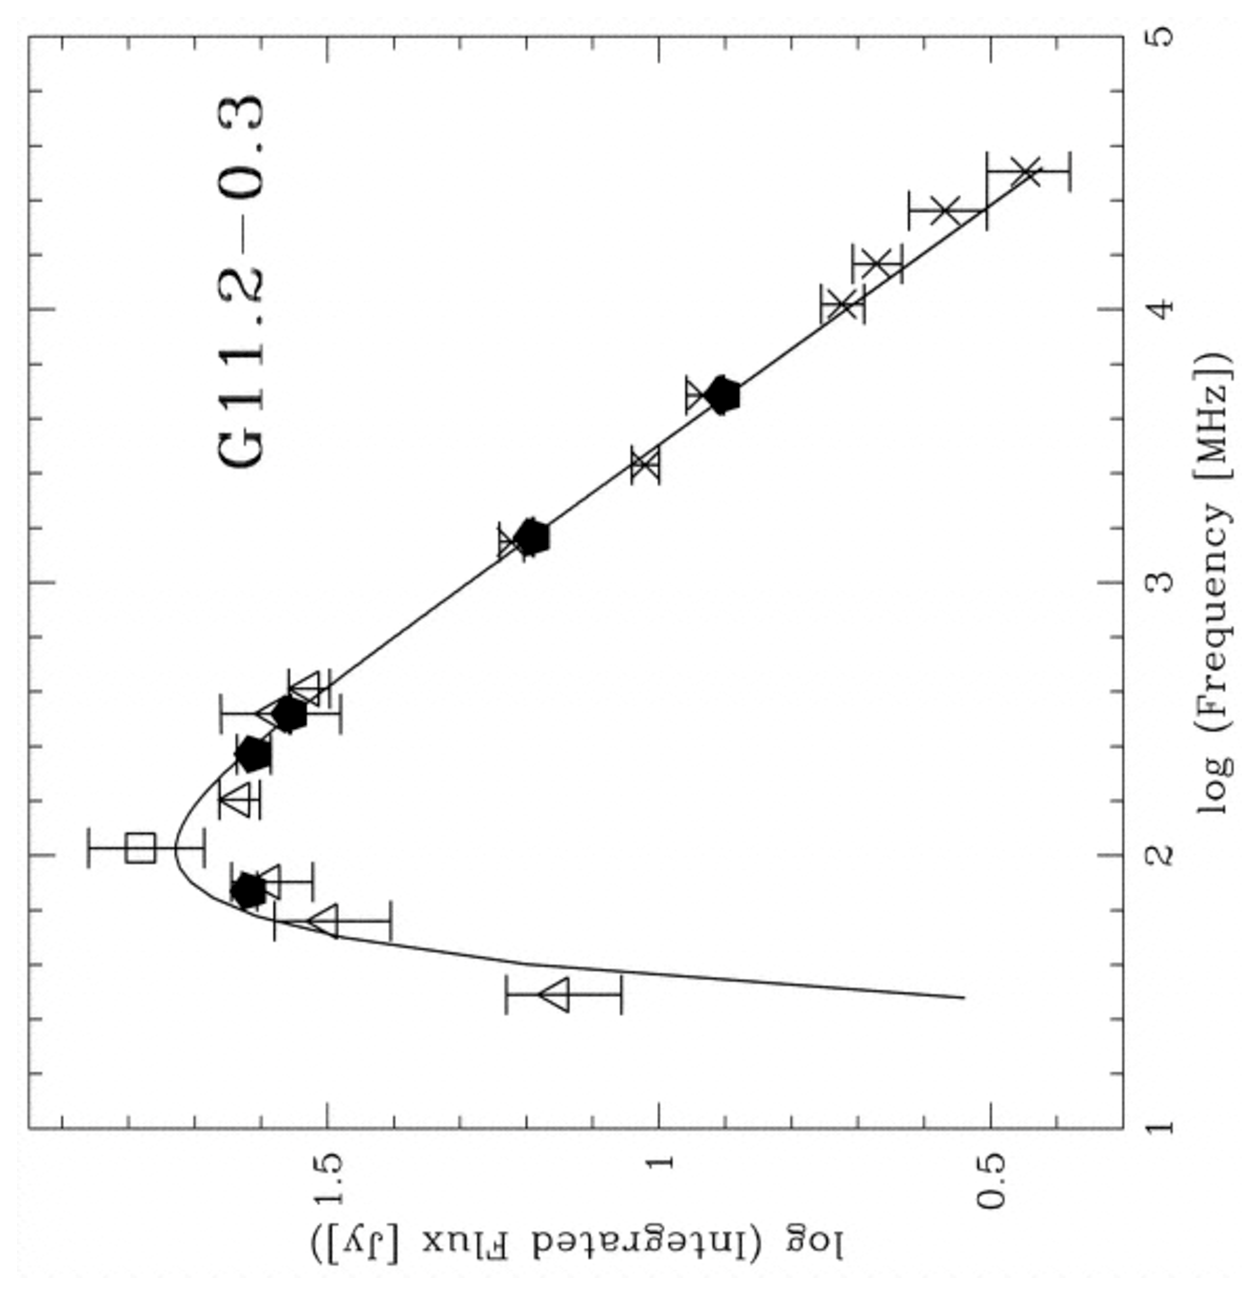
\includegraphics[width=3.4in]{fig2.eps} 
		\caption{M-M graph to test general relativity using PK parameters for PSR J0737-3039. Taken from \cite{james16}}
		\label{fig2}
	\end{center}
\end{figure}

 
\subsection{Eclipsing of A and the Penetration of B's Magnetosphere}

At conjunction, the line of sight of the two pulsars is within 0.15 ls of each other. As they further advance in their orbits, A is completely eclipsed by B and the line of sight of A sweeps through the magnetosphere of B. \cite{lyn04} suggested that studying the changes in radio transmission during this process can lead to understanding the physical conditions of B's magnetosphere, giving a better understanding of the plasma density and  magnetic field structure. Analysis of flux densities(figure 3) revealed an occultation of A occurs that lasts around 20s ot 30s. The spin-down energy loss of A being 3000 times greater than that of B, and the energy density of the relativistic wind from A being two orders of magnitude larger than B's, it was suggested that the wind from A will penetrate deep into B's magnetosphere. In fact, it was found that at radii greater than 40\% of the light cylinder of B, the energy field of A dominates. Because of this, the penetration of wind from A into that of B was hypothesized to be dependent on their relative orientation. This dependence was cited as the cause for fluctuations in B's flux densities over time. 

% CUP work flow only accepts EPS -- not PDF, JPG, etc.
\begin{figure}[h!]
	\begin{center}
		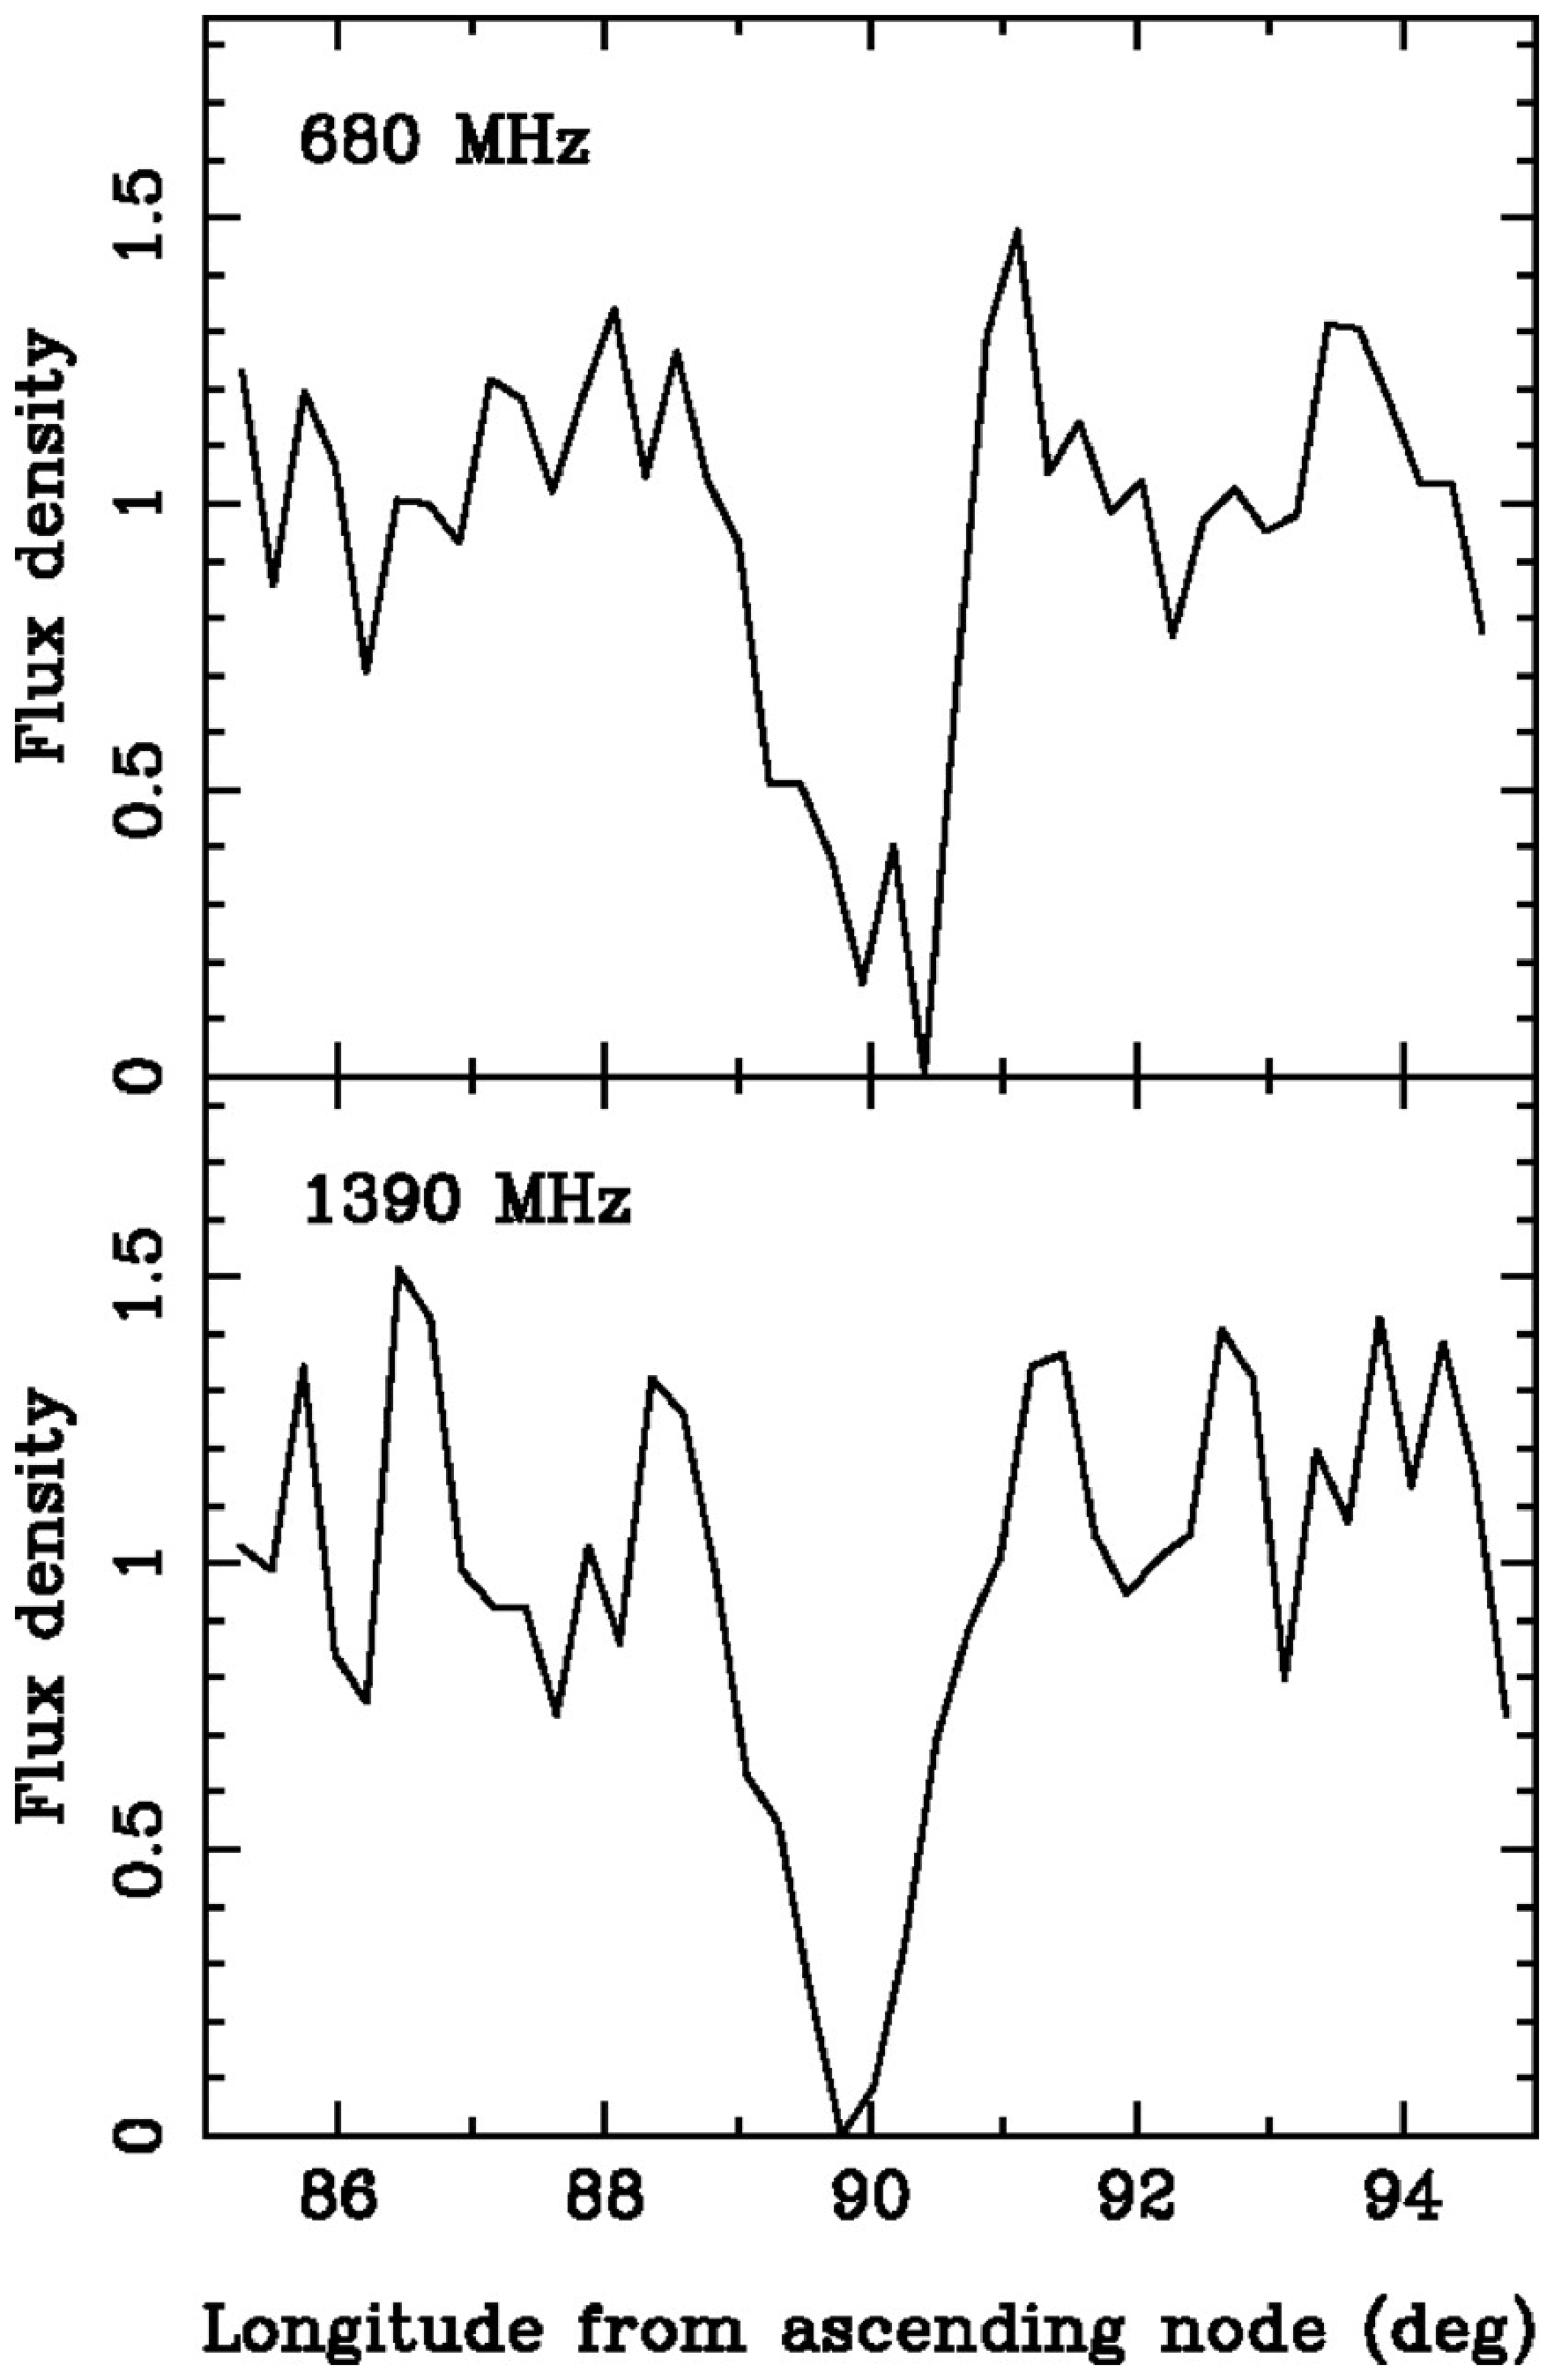
\includegraphics[width=3.4in]{fig3.eps} 
		\caption{The variation in flux density of A (in arbitrary units) at 680 and 1390 MHz, around superior conjunction (i.e., longitude 90°). The data are presented with 5-s time resolution and show the eclipse of the pulsar by the magnetosphere of B.Image and description taken from \cite{lyn04} }
		\label{fig3}
	\end{center}
\end{figure}

% CUP work flow only accepts EPS -- not PDF, JPG, etc.
\begin{figure}[h!]
	\begin{center}
		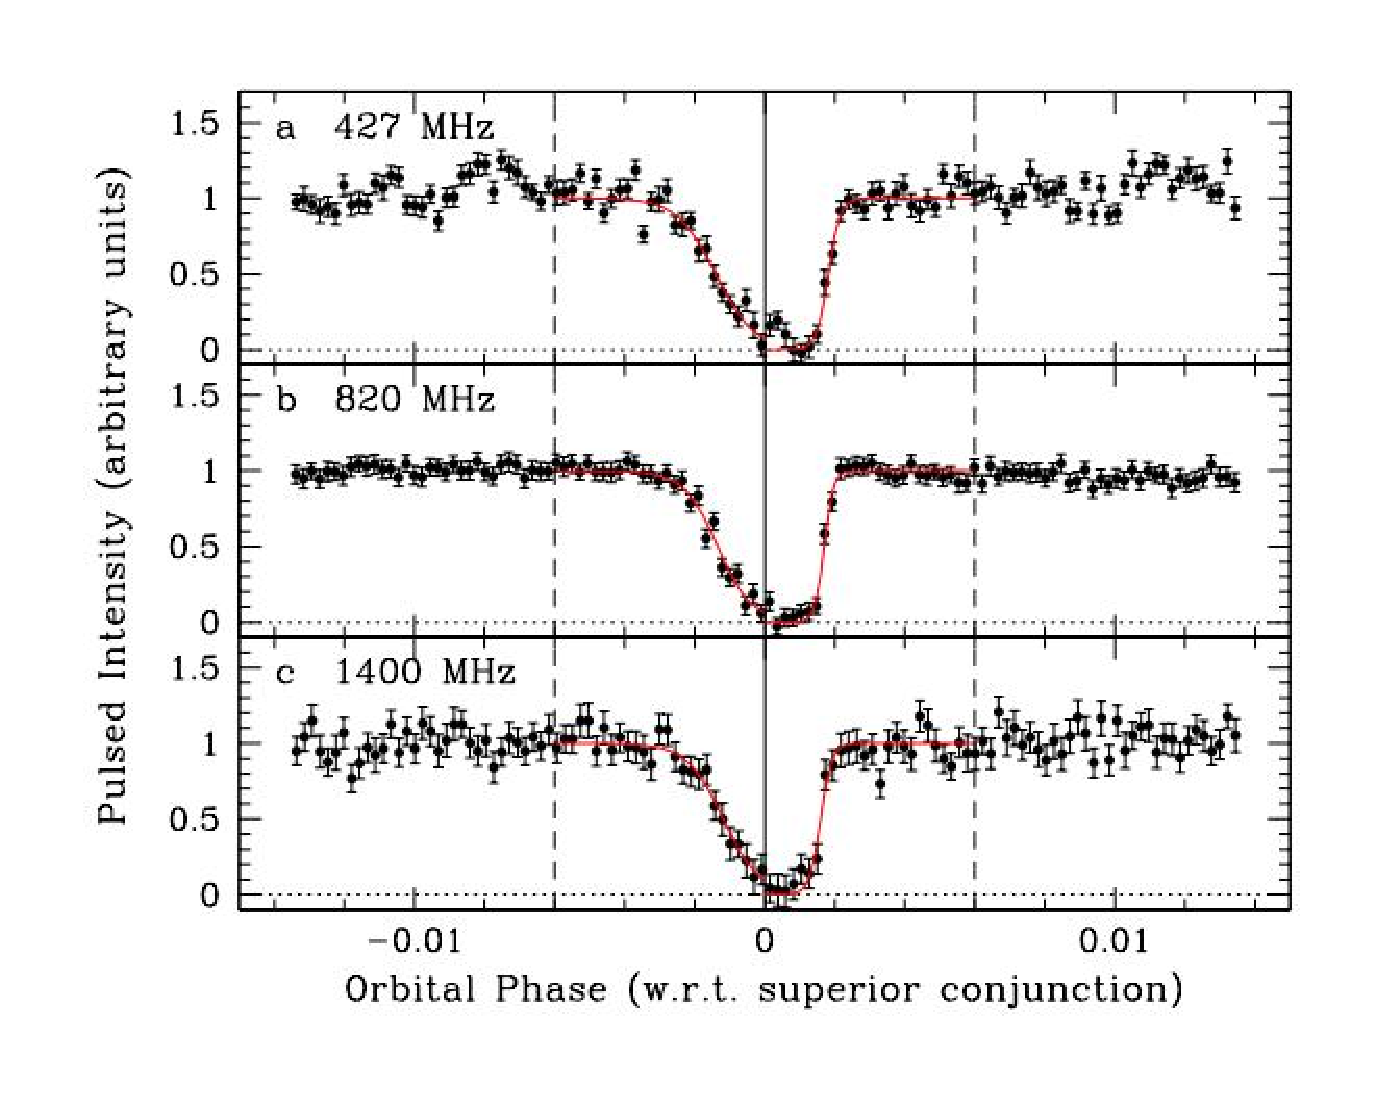
\includegraphics{fig4.eps} 
		\caption{Pulsar A eclipse light curves. Each point represents 2 s of data; the shown curve
			is 4-min in duration, centered on conjunction. The x-axes are orbital phase with respect to
			conjunction. The y-axes are pulsed flux, normalized such that the pre-eclipse flux is unity.
			The panels are for (a) 427 MHz, (b) 820 MHz, and (c) 1400 MHz. The solid vertical line
			indicates conjunction and the horizontal dotted lines show 0 flux. Vertical dashed lines at
			$\phi$ = −0.006, +0.006 indicate the range of data fitted. The best-fit ingress and egress model
			curves are shown as solid lines. Figure and its description is from \cite{kapsi04} }
		\label{fig4}
	\end{center}
\end{figure}

\cite{kapsi04} observed the eclipsing of A in further detail using measurements from the Green Bank Telescope at 427,820, and 1400 MHz.  The light curves(figure 4) obtained showed that  the eclipse ingress is longer than the eclipse egress. The observation also confirmed the eclipse model put forth by \cite{arons05} (Note that Aaron's paper was unpublished when GBT's results were published). A's wind confines B's magnetosphere on the side facing A, compressing it. While the part of B's magnetosphere opposite to the side facing A develops a magnetotail. The heating up of A's wind plasma by the bow shock developed was hypothesized to rise of synchroton absorption, leading to A's eclipse. The rotation of B's magnetosphere was held accountable for the eclipse asymmetries. It was also postulated that at frequencies around 5-10GHz, the eclipse will clear. 

\subsection{Implications for the DNS Merger Rates}

As already explained, PSR J0737-3039 has provided a rigorous testing ground for gravitation theories. However, it must be noted that the very first important result obtained from observations of stars in this system led to setting new limits on the DNS merger rates. A relativistic DNS system such as this is expected to result in a gravitational wave burst and a neutron star/black hole depending on the properties of stars in the system \cite{lipun04}. 

When PSR J0737-3039 was discovered, its lifetime was first found to be 85Myr. Since PSR B1913+16 and PSR B1534+12 were the highest contributors to merger rate calculations at that time, the lifetime and luminosity of PSR J0737-3039 was compared with these two stars. Since the lifetime of PSR B1913+16 was 300 My, PSR J0737-3039's discovery significantly affected the DNS merger rate estimates. With these considerations, \cite{b03} calculated that PSR J0737-3039 caused a decrease in DNS merger rates by one order of magnitude. So the DNS merger rate went from $10^{-5}$ year$^{-1}$ to $10^{-4}$ year$^{-1}$.












\begin{thebibliography}{}

\bibitem[Burgay et al. (2003)]{b03} Burgay, M., N. D’Amico, A. Possenti, R. N. Manchester, A. G. Lyne, B. C. Joshi, M. A. McLaughlin, et al. 2003. Nature 426 (6966): 531–33. https://doi.org/10.1038/nature02124.

\bibitem[Lyne (2006)]{lyn06} Lyne, A.G., 2006. Chinese Journal of Astronomy and Astrophysics Supplement 6, 162.

\bibitem[Lyne et al. (2004)]{lyn04} Lyne, A.G., Burgay, M., Kramer, M., Possenti, A., Manchester, R.N., Camilo, F., McLaughlin, M.A., Lorimer, D.R., D’Amico, N., Joshi, B.C., Reynolds, J., Freire, P.C.C., 2004. Science 303, 1153–1157.

\bibitem[Kramer and Wex (2009)]{kwex09} Kramer, M., Wex, N., 2009. Class. Quantum Grav. 26, 073001.

\bibitem[Kaspi et al., (2004)]{kapsi04} Kaspi, V.M., Ransom, S.M., Backer, D.C., Ramachandran, R., Demorest, P., Arons, J., Spitkovsky, A., 2004. The Astrophysical Journal 613, L137–L140.

\bibitem[Lyutikov and Thompson, (2005)]{Lyut05} Lyutikov, M., Thompson, C., 2005. ApJ 634, 1223.

\bibitem[Arons et al. (2005)]{arons05} Arons, J., C. Backer, D., Spitkovsky, A., M. Kaspi, V., 2005. 95.

\bibitem[James et al. (2016)]{james16}  James Justin Condon, Scott M. Ransom, 2016. 6 Pulsars‣ Essential Radio Astronomy [WWW Document]. URL https://www.cv.nrao.edu/~sransom/web/Ch6.html (accessed 10.17.18).

\bibitem[Lipunov (2004)]{lipun04} Lipunov, V.M., 2004. arXiv:astro-ph/0406502.




\end{thebibliography}


\end{document}
